\begin{center}
\begin{tikzpicture}
    \node[anchor=south west,inner sep=0] (image)  at (0,0) {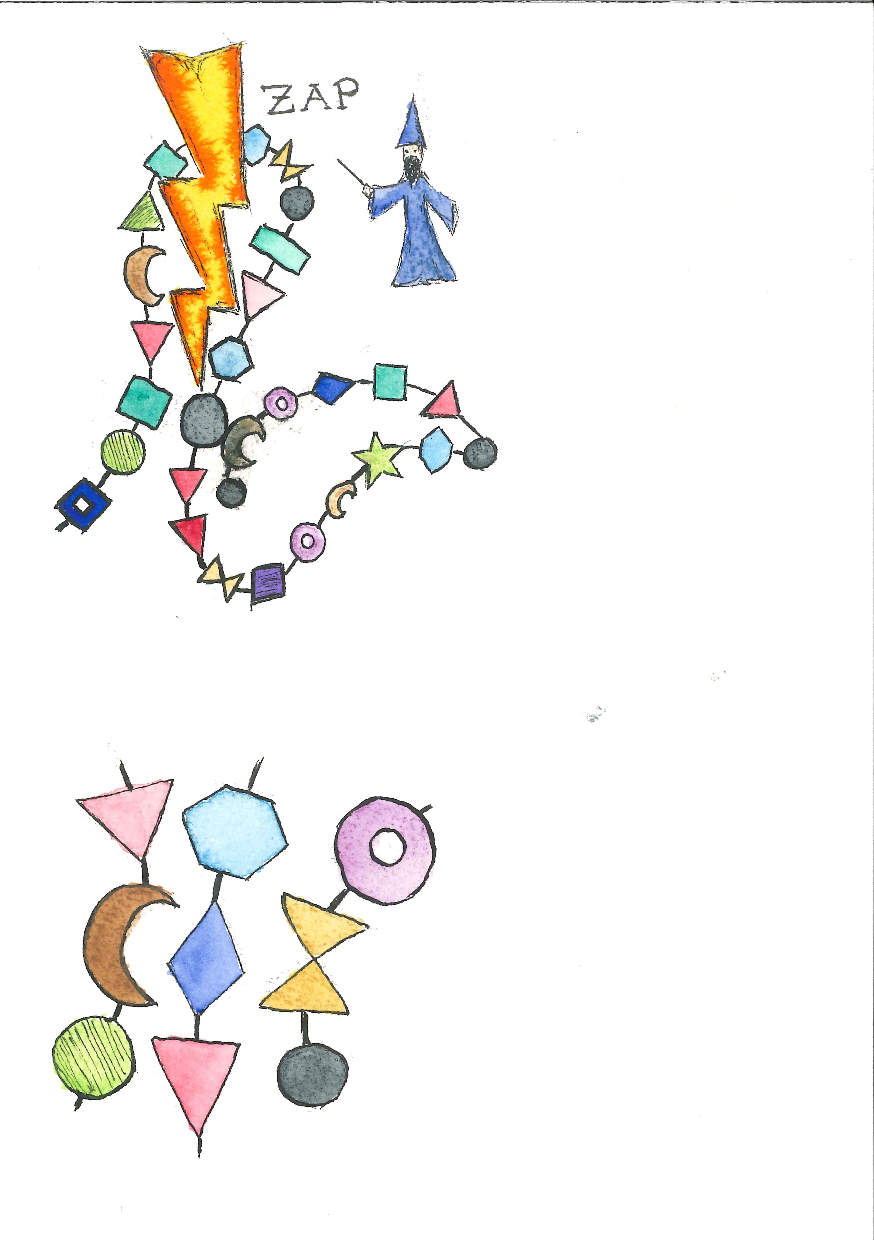
\includegraphics[trim={2mm, 2mm, 2mm, 2mm}, width=0.995\pagewidth]{scans/pg_0005.pdf}};


    \begin{scope}[x={(image.south east)},y={(image.north west)}]
        \if\helplines1
        	\draw[help lines,xstep=.1,ystep=.1] (0,0) grid (1,1);
        \fi
        \node[align=justify, anchor=north west, text width = 0.32\pagewidth](0) at (0.6, 0.9) {\english{Proteins are tightly packed inside, so when, for whatever reason, an amino acid is mutated,}};
        
        \node[align=justify, anchor=north west, text width = 0.4\pagewidth](0) at (0.52, 0.4) {\english{likely other amino acids close in space will also change to preserve the chemical properties.
        
        \doindent The amino acids that “touch" each other are called \emph{contacts}.}};
        
        % % % % % % % % % % % % %
        \node[align=justify, anchor=north west, text width = 0.32\pagewidth](0) at (0.6, 0.76) {\spanish{Las proteínas están empaquetadas muy densamente, así que cuando, por cualquier razón, un aminoácido muta,}};
        \node[align=justify, anchor=north west, text width = 0.4\pagewidth](0) at (0.52, 0.2) {\spanish{es probable que otros aminoácidos cercanos en el espacio también cambien, para preservar las propiedades energéticas.
                
        \doindent Los aminoácidos que <<se tocan>> se llaman \emph{contactos}.}};
        
        
    \end{scope}

\end{tikzpicture}
\end{center}